
% Include LaTeX packages
\documentclass[conference]{styles/acmsiggraph}
\usepackage{comment} % enables the use of multi-line comments (\ifx \fi)
\usepackage{fullpage}
\usepackage{enumitem}
\usepackage{amsmath,amsthm,amssymb}
\usepackage{listings}
\usepackage{minted}
\usepackage{graphicx}
\usepackage{etoolbox}
\usepackage{verbatim}
\usepackage[dvipsnames]{xcolor}
\usepackage{fancyvrb}
\usepackage{hyperref}
\usepackage{menukeys}
\usepackage{titlesec}
\usepackage{csquotes}
\usepackage{placeins}
\usepackage{algorithm} 
\usepackage{algpseudocode}
\usepackage{booktabs}
\usepackage{unicode-math}
\newcommand{\?}{\stackrel{?}{=}}
\renewcommand\qedsymbol{$\blacksquare$}

% Set additional LaTeX options
\setlength{\parskip}{.8mm}
\setcounter{MaxMatrixCols}{20}
\hypersetup{
	colorlinks=true,
	urlcolor=[rgb]{0.97,0,0.30},
	anchorcolor={0.97,0,0.30},
	linkcolor=black,
	filecolor=[rgb]{0.97,0,0.30},
}

% Define title, author, and affiliation information
\title{\huge Programming Assignment 1 \\ \LARGE {CS124: Data Structures and Algorithms \\ Prof. Mitzenmacher}}
\author{\Large Benny Paris \& Dhilan Ramaprasad \\
bparis@college.harvard.edu\\dhilanramaprasad@college.harvard.edu}
\pdfauthor{Dhilan/Benny}

% Redefine \VerbatimInput
\RecustomVerbatimCommand{\VerbatimInput}{VerbatimInput}%
{fontsize=\footnotesize,
 %
 frame=lines, % top and bottom rule only
 framesep=2em, % separation between frame and text
 rulecolor=\color{Gray},
 %
 label=\fbox{\color{Black}\textbf{OUTPUT}},
 labelposition=topline,
 %
 commandchars=\|\(\), % escape character and argument delimiters for commands within the verbatim
 commentchar=* % comment character
}

% Set addditional formatting options
\titlespacing*{\section}{0pt}{5.5ex plus 1ex minus .2ex}{2ex}
\titlespacing*{\subsection}{0pt}{3ex}{2ex}
\setcounter{secnumdepth}{4}
\renewcommand\theparagraph{\thesubsubsection.\arabic{paragraph}}
\newcommand\subsubsubsection{\paragraph}

% Define a convenient norm symbol
\newcommand{\norm}[1]{\left\lVert#1\right\rVert}
\renewcommand{\vec}[1]{\mathbf{#1}}

% Define a macro for hiding answers
\newbool{hideanswers} \setbool{hideanswers}{false}
\newenvironment{answer}{}{}
\ifbool{hideanswers}{\AtBeginEnvironment{answer}{\comment} %
\AtEndEnvironment{answer}{\endcomment}}{}

% Define text formatting for points and normals
\newcommand{\points}[1]{\hfill \normalfont{(\textit{#1pts})}}
\newcommand{\pointsin}[1]{\normalfont{(\textit{#1pts})}}







%%%%%%%%%%%%%%%%%%%%%%%%%%%%%%%%%%%%%%%
%%%%%%%%%%%%%%%%%%%%%%%%%%%%%%%%%%%%%%%
%%%%%%%%%%%%%%%%%%%%%%%%%%%%%%%%%%%%%%%
%%%%%%%%%%%%%%%%%%%%%%%%%%%%%%%%%%%%%%%
%%%%%%%%%%%%%%%%%%%%%%%%%%%%%%%%%%%%%%%

         %  START HERE  %

%%%%%%%%%%%%%%%%%%%%%%%%%%%%%%%%%%%%%%%
%%%%%%%%%%%%%%%%%%%%%%%%%%%%%%%%%%%%%%%
%%%%%%%%%%%%%%%%%%%%%%%%%%%%%%%%%%%%%%%
%%%%%%%%%%%%%%%%%%%%%%%%%%%%%%%%%%%%%%%
%%%%%%%%%%%%%%%%%%%%%%%%%%%%%%%%%%%%%%%

\begin{document}
\maketitle

\section{Raw Results:} \label{section:RESULTS}
We ran \textbf{at least 5 trials} for each row of each of the proceeding tables.  \enquote{MST Weight} was averaged among the trials; whereas, \enquote{Max Weight} was selected as the maximum edge-weight in any MST produced by any of our trials for the given $n$. \enquote{Run Time} varies slightly from projections discussed in Section \ref{section:RUNTIME} due to use of two computers and differing times of trial runs (i.e., during the day trials were running in the background while our laptops were being used).
%1D
\begin{table}[htbp]
  \centering
  \caption{1-Dimension Trials}
    \begin{tabular}{cccc}
    \toprule
    \textbf{n} & \textbf{MST Weight (Averaged Total)} & \textbf{Max Weight} & \textbf{Run Time (s)} \\
    \midrule
    128   & 1.15267 & 0.0685441 & 0.0018396 \\
    256   & 1.19467 & 0.0274457 & 0.0050726 \\
    512   & 1.15699 & 0.0171285 & 0.0168936 \\
    1024  & 1.21067 & 0.00783824 & 0.0642364 \\
    2048  & 1.18916 & 0.00466485 & 0.248078 \\
    4096  & 1.2114 & 0.00199551 & 0.967547 \\
    8192  & 1.2033 & 0.00156452 & 4.08914 \\
    16384 & 1.21069 & 0.00075186 & 15.8118 \\
    32768 & 1.20264 & 0.00037903 & 61.9953 \\
    65536 & 1.20306 & 0.0001824 & 247.646 \\
    131072 & 1.20312 & 9.612E-05 & 1001.3 \\
    262144 & 1.20051 & 5.575E-05 & 4050.075 \\
    \bottomrule
    \end{tabular}%
  \label{tab:addlabel}%
\end{table}%


%2D
\begin{table}[htbp]
  \centering
  \caption{2-Dimension Trials}
    \begin{tabular}{cccc}
    \toprule
    \textbf{n} & \textbf{MST Weight (Averaged Total)} & \textbf{Max Weight} & \textbf{Run Time (s)} \\
    \midrule
    128   & 7.49185 & 0.153954 & 0.0018658 \\
    256   & 10.6118 & 0.113735 & 0.0054642 \\
    512   & 14.8725 & 0.0937277 & 0.0196978 \\
    1024  & 21.1721 & 0.0622288 & 0.0752236 \\
    2048  & 29.5789 & 0.0399356 & 0.283358 \\
    4096  & 41.7103 & 0.0316518 & 1.08435 \\
    8192  & 58.8472 & 0.0236516 & 4.68257 \\
    16384 & 83.0779 & 0.019116 & 17.4895 \\
    32768 & 117.491 & 0.0115361 & 69.9517 \\
    65536 & 165.992 & 0.00816879 & 283.006 \\
    131072 & 234.617 & 0.00709486 & 1159.09 \\
    262144 & 331.576 & 0.00408205 & 4828.96 \\
    \bottomrule
    \end{tabular}%
  \label{tab:addlabel}%
\end{table}%


% 3D
\begin{table}[htbp]
  \centering
  \caption{3-Dimension Trials}
    \begin{tabular}{cccc}
    \toprule
    \textbf{n} & \textbf{MST Weight (Averaged Total)} & \textbf{Max Weight} & \textbf{Run Time (s)} \\
    \midrule
    128   & 17.4721 & 0.309436 & 0.002182 \\
    256   & 27.3752 & 0.24907 & 0.0065144 \\
    512   & 43.7455 & 0.204125 & 0.0239144 \\
    1024  & 67.7711 & 0.157856 & 0.0904782 \\
    2048  & 107.024 & 0.122984 & 0.341465 \\
    4096  & 168.773 & 0.111061 & 1.32476 \\
    8192  & 267.515 & 0.0886609 & 5.71163 \\
    16384 & 422.142 & 0.0668047 & 21.5808 \\
    32768 & 669.334 & 0.0537248 & 87.4818 \\
    65536 & 1059.76 & 0.0406939 & 357.261 \\
    131072 & 1675.25 & 0.0320848 & 1456.37 \\
    262144 & 2659.65 & 0.0264553 & 5484.98 \\
    \bottomrule
    \end{tabular}%
  \label{tab:addlabel}%
\end{table}%

% 4D
\begin{table}[htbp]
  \centering
  \caption{4-Dimension Trials}
    \begin{tabular}{cccc}
    \toprule
    \textbf{n} & \textbf{MST Weight (Averaged Total)} & \textbf{Max Weight} & \textbf{Run Time (s)} \\
    \midrule
    128   & 28.8833 & 0.426479 & 0.0025936 \\
    256   & 47.3244 & 0.375659 & 0.0071628 \\
    512   & 78.6795 & 0.307146 & 0.0269444 \\
    1024  & 130.069 & 0.273687 & 0.102985 \\
    2048  & 216.778 & 0.280314 & 0.39541 \\
    4096  & 360.769 & 0.179831 & 1.61305 \\
    8192  & 604.499 & 0.18349 & 6.3846 \\
    16384 & 1009.19 & 0.127061 & 25.9584 \\
    32768 & 1689.12 & 0.115782 & 105.228 \\
    65536 & 2828.95 & 0.0987119 & 430.896 \\
    131072 & 4738.05 & 0.0847639 & 1771.44 \\
    262144 & 7955.135 & 0.0656702 & 6137.14 \\
    \bottomrule
    \end{tabular}%
  \label{tab:addlabel}%
\end{table}%
\FloatBarrier


\section{Finding $f(n)$:}
\subsection{Our Results:}
To find $f(n)$, the function of the average graph size with respect to the number of nodes, we will use the preceding data-sets (see Section \ref{section:RESULTS}) which show the average MST size for the four options of dimensions.  

\subsection{First Look:}
We will take a cursory glance at the data to find indicators for curve-fitting, i.e., functional forms to test and expectations of parsimony and fidelity.  

\subsubsection{1-D Data:}
From Figure \ref{fig:1Dvn} (the plot of average MST size for the 1-D case versus $n$), made in \textbf{R}, we see that the points do not seem to vary much with $n$.  The only effect that increased $n$ seems to carry is decreased variance, which makes sense; our random number generator might give us results that are unexpected or extreme for very small $n$, but by the \textit{Law of Large Numbers}, we know that random variables are less and less likely to be obscured by random effects as our sample size grows.  Now, we do know that our values for $n$ are spaced apart, being consecutive powers of 2; as such, we examine the $\log$ of $n$ as a potential independent variable.  The plot for the log relationship is shown below (see Figure \ref{fig:1D_log}); a linear appearance to such a plot would imply a relationship. 


\begin{figure}[h!]
    \centering
    \begin{subfigure}
    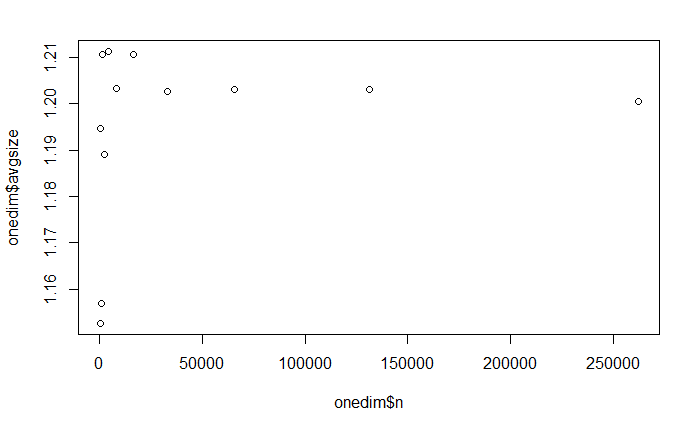
\includegraphics[width=0.4\textwidth]{1dplot124.png}
    \caption{Average MST Size v. $n$}
    \label{fig:1Dvn}
    \end{subfigure}
    \begin{subfigure}
    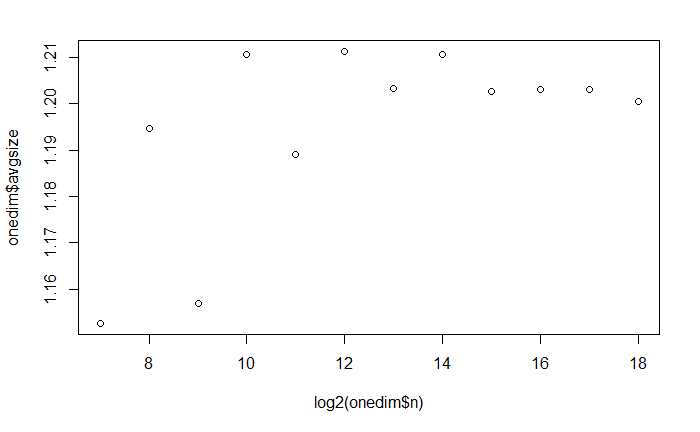
\includegraphics[width=0.4\textwidth]{1dplotlog.png}
    \caption{Average MST Size v. $\mathbf{log(n)}$}
    \label{fig:1D_log}
    
    \end{subfigure}
\end{figure}
\FloatBarrier % this makes sure the image goes right here.

We see that these plots do not show much of a clear linear relationship whatsoever; it would seem that our average MST size may not be correlated with $n$ at all.  We will examine the data more closely to support this in our Data Analysis Subsection (see Section \ref{section:DATAANALYSIS}).


\subsubsection{2-D Data:} 

Below (see Figure \ref{fig:2DvN}) is the average MST size plotted against $n$ for 2-Dimensional trials (i.e., inside the unit square). 

\begin{figure}[h!]
    \centering
    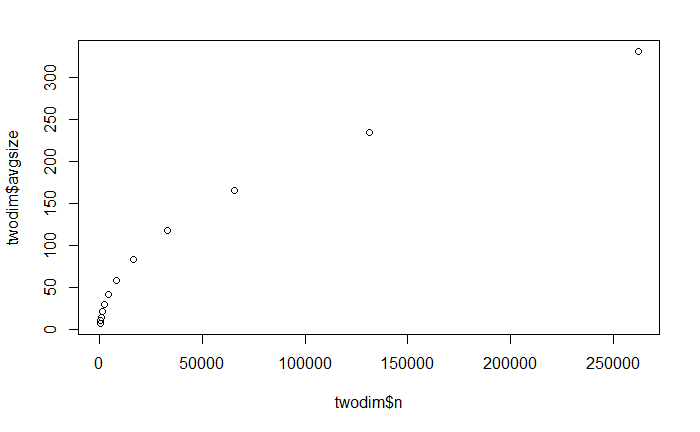
\includegraphics[width=0.4\textwidth]{2dplotlinear.png}
    \caption{On the y axis is the average MST size; the x axis is $n$}
    \label{fig:2DvN}
\end{figure}
\FloatBarrier % this makes sure the image goes right here.

We see the above looks a log-response, so we will try taking $log(n)$ and plot that as the $x$ axis (see Figure \ref{fig:2D_log}).  The goal is for the plot below to look \textbf{as linear as possible}, because linearity of the plot allows us to use linear regression to solve for the correct constant factors.  

\begin{figure}[h!]
    \centering
    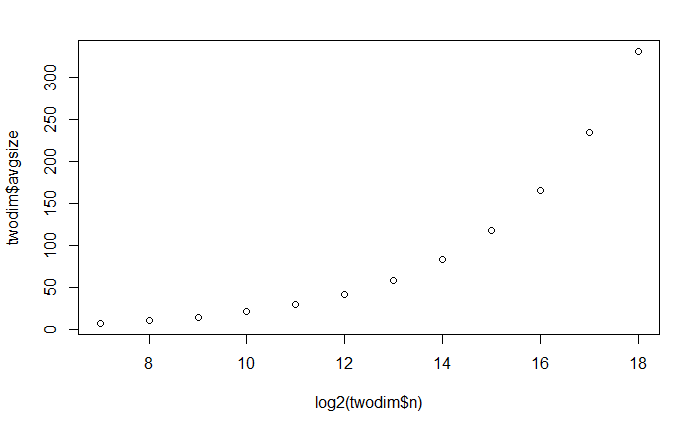
\includegraphics[width=0.4\textwidth]{2dplotlog.png}
    \caption{Average MST size v. $\mathbf{log(n)}$}
    \label{fig:2D_log}
\end{figure}
\FloatBarrier % this makes sure the image goes right here.

Figure \ref{fig:2D_log} has a problem; it clearly does not look linear.  Instead, it looks like $y\sim 2^x$ for $x=log(n)$.  But this is even worse, because, of course, we are back to our $y\sim x$ graph, which was clearly not correct.  So, now, we will try to do something outside of $\log$; perhaps the first plot showed not a $\log$ relationship, but a root relationship (see Figure \ref{fig:2D_root}):

\begin{figure}[h!]
    \centering
    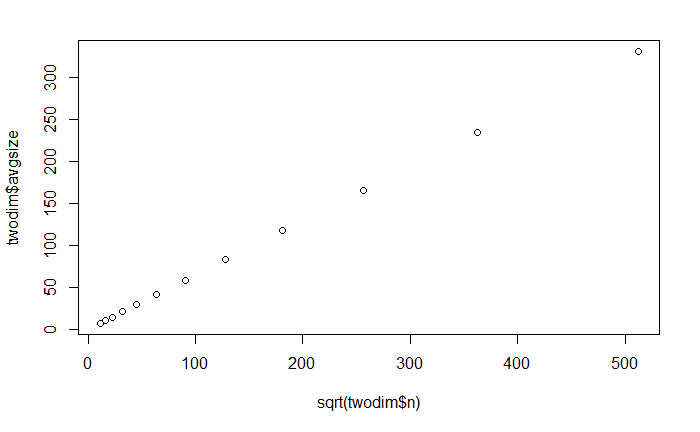
\includegraphics[width=0.4\textwidth]{2dplotsqrt.png}
    \caption{Average MST size v. $\mathbf{\sqrt{n}}$}
    \label{fig:2D_root}
\end{figure}
\FloatBarrier % this makes sure the image goes right here.

Wow!  As we can see, Figure \ref{fig:2D_root} looks incredibly linear.  We will pursue this for our data analysis later on.  

\subsubsection{3-D Data:}

We see our linear and log-linear plots look basically the same as in the $2-D$ case:

\begin{figure}[h!]
    \centering
    
    \begin{subfigure}
     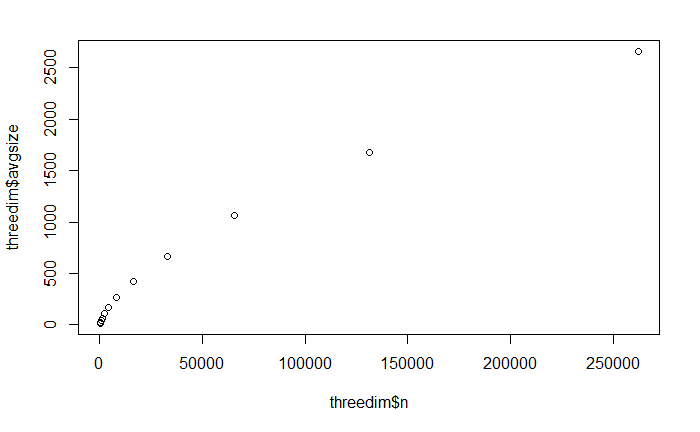
\includegraphics[width=0.4\textwidth]{3dplotlinear.png}
    \caption{Average MST Size v. $n$}
    \label{fig:3Dvn}
    \end{subfigure}
    
    \begin{subfigure}
    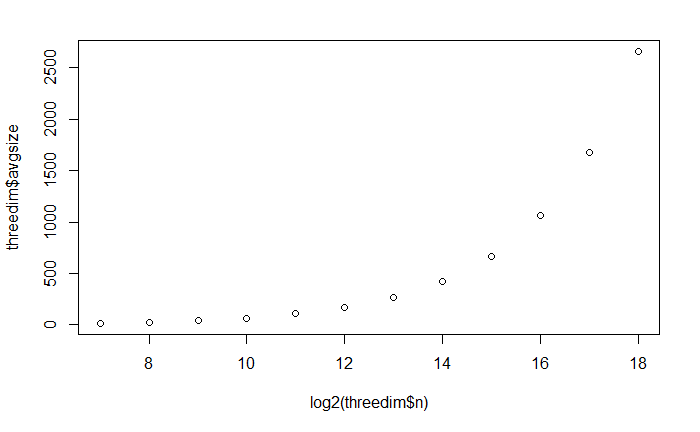
\includegraphics[width=0.4\textwidth]{3dplotlog.png}
    \caption{Average MST Size v. $\mathbf{log(n)}$}
    \label{fig:3DvLOG}
    \end{subfigure}
\end{figure}
\FloatBarrier % this makes sure the image goes right here.

However, we see that the square root plot (see Figure \ref{fig:3DvROOT}) does not look as linear as before:

\begin{figure}[h!]
    \centering
    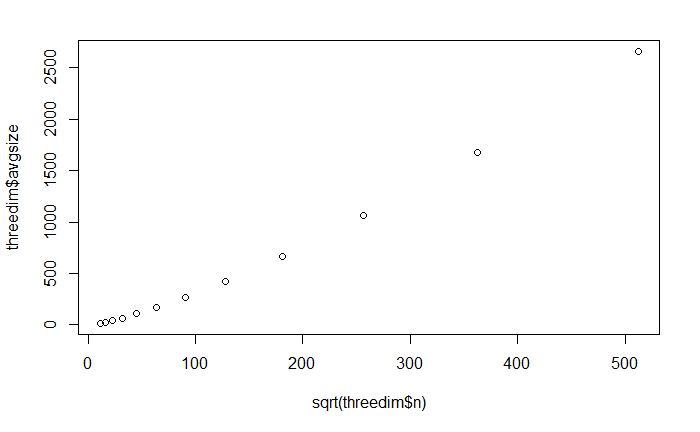
\includegraphics[width=0.4\textwidth]{3dplotsqrt.png}
    \caption{Average MST size v. $\mathbf{\sqrt{n}}$}
    \label{fig:3DvROOT}
\end{figure}
\FloatBarrier % this makes sure the image goes right here.

Figure \ref{fig:3DvROOT} does not look \textit{too} curved, but we should be concerned.  We can examine whether this curve is ``real'' by our \textit{residual plot}.  A residual plot shows the difference between $f(n)$ and $\hat{f}(n)$. According to the statistical models behind $lm$, our residual should be some $\epsilon \sim \mathcal{N}(0,\sigma^2)$, i.e., a plot of our residuals should look random and centered around $0$. If our residual plot seems to have a functional form or shape to it, we probably have a bad functional form.  Our \textbf{R} output for the $lm$ function, run on the square root model for the 3-D data, gives the following residual plot (see Figure \ref{fig:ROOTresid}):

\begin{figure}[h!]
    \centering
    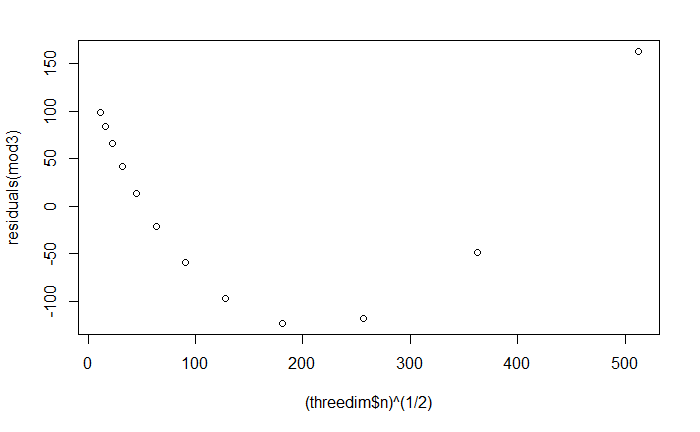
\includegraphics[width=0.4\textwidth]{3dplotsres.png}
    \caption{Residuals v. $\mathbf{\sqrt{n}}$}
    \label{fig:ROOTresid}
\end{figure}
\FloatBarrier % this makes sure the image goes right here.

Figure \ref{fig:ROOTresid} has an obvious shape and varies between around 150 to below $-100$, a pretty high range considering our $y$ values go to around 2000. So, we will look at a different functional form.  The square root was close, so we examine, for $n^{2/3}$, both the regular plot (Figure \ref{fig:3Dv23}) and the residual plot (Figure \ref{fig:3D23res}):

\begin{figure}[h!]
    \centering
    \begin{subfigure}
    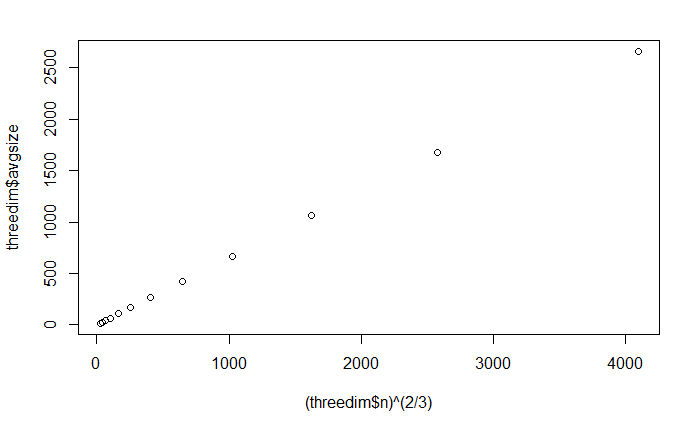
\includegraphics[width=0.4\textwidth]{3dplot23.png}
    \caption{Average MST size v. $\mathbf{n^{2/3}}$}
    \label{fig:3Dv23}
    \end{subfigure}
    \begin{subfigure}
    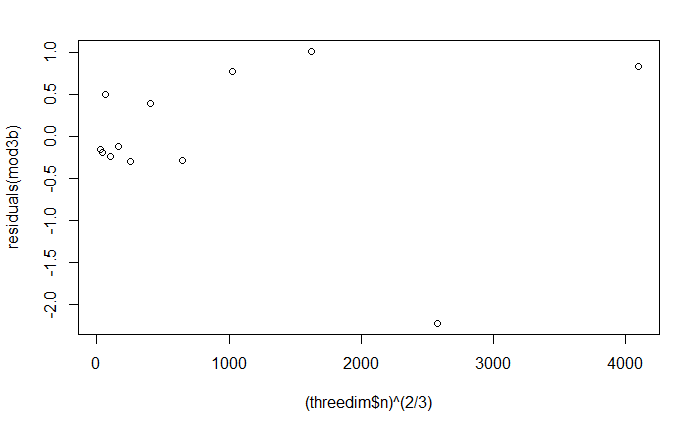
\includegraphics[width=0.4\textwidth]{3dplot23res.png}
    \caption{Residuals v. $\mathbf{n^{2/3}}$}
    \label{fig:3D23res}
    \end{subfigure}
\end{figure}
\FloatBarrier % this makes sure the image goes right here.


\subsubsection{4-D Data:}

We notice a pattern emerging, and so we will test only the $\sqrt{n}$, $n^{2/3}$, and (seeing a pattern, namely, $0/1, 1/2, 2/3, 3/4, 4/5, \ldots$) $3/4$.  Below are the plots for these functions:
\begin{figure}[h!]
    \centering
    \begin{subfigure}
     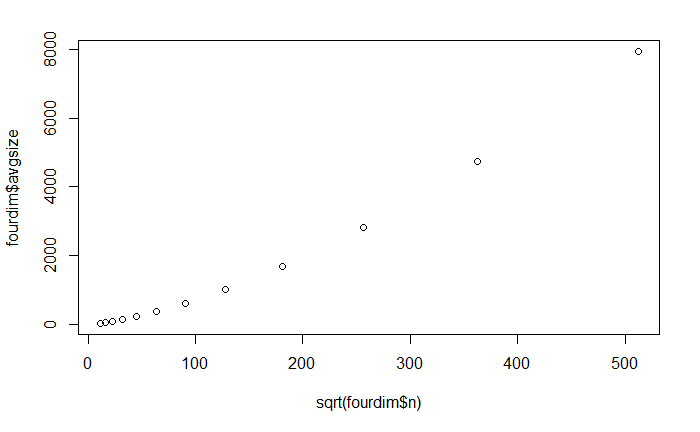
\includegraphics[width=0.4\textwidth]{4dplotsqrt.png}
    \caption{Average MST size v. $\mathbf{\sqrt{n}}$}
    \label{4dSQRT}
    \end{subfigure}
    \begin{subfigure}
    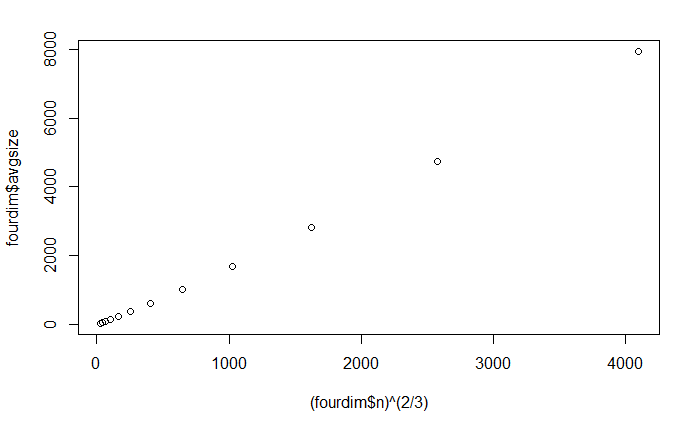
\includegraphics[width=0.4\textwidth]{4dplot23.png}
    \caption{Average MST size v. $\mathbf{n^{2/3}}$}
    \label{}
    \end{subfigure}
    \begin{subfigure}
    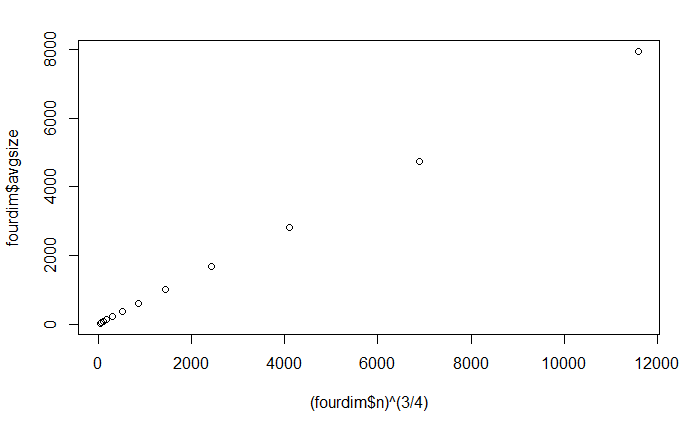
\includegraphics[width=0.4\textwidth]{4dplot34.png}
    \caption{Average MST size v. $\mathbf{n^{3/4}}$}
    \label{}
    \end{subfigure}
\end{figure}
\FloatBarrier % this makes sure the image goes right here.


We see that $3/4$ looks best, but to avoid over-fitting, we will examine the residual plots of both $2/3$ and $3/4$:

\begin{figure}[h!]
    \centering
    \begin{subfigure}
    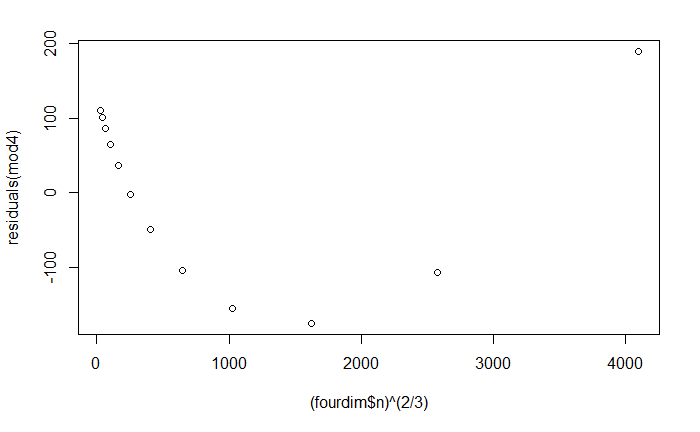
\includegraphics[width=0.4\textwidth]{4dplot23res.png}
    \caption{Residuals v. $\mathbf{n^{2/3}}$}
    \label{4Dresid23}
    \end{subfigure}
    \begin{subfigure}
    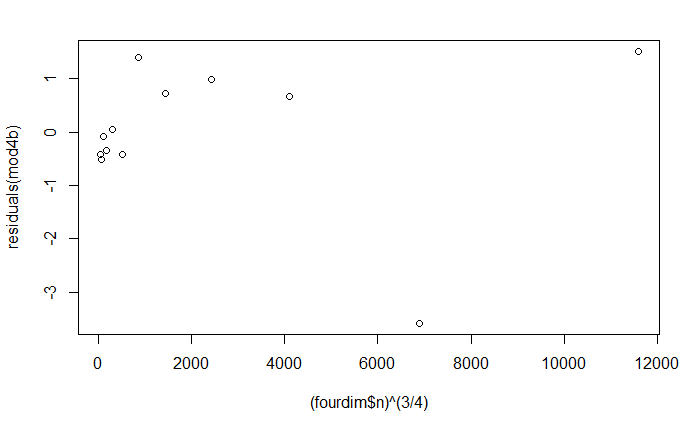
\includegraphics[width=0.4\textwidth]{4dplot34res.png}
    \caption{Residuals v. $\mathbf{n^{3/4}}$}
    \label{4dresid34}
    \end{subfigure}
\end{figure}
\FloatBarrier % this makes sure the image goes right here.

We see that the $2/3$ residual plot (see Figure \ref{4Dresid23}) clearly has a functional form and a very large range.  However, the $3/4$ plot (see Figure \ref{4dresid34}) also has something of a functional form, vaguely seeming periodic.  However, its range is so small--around $-5 to 5$--that we properly understand this to be periodicity of our Mersenne Twister pseudo-random number generator.  We will choose $3/4$ as the power of $n$ for the 4-D function.  

\subsection{Data Analysis and $f(n)$:} \label{section:DATAANALYSIS}

\subsubsection{1-D:}
We will compare the p-values of the linear, log, and constant models to support our choice of the latter.  P-values give us an idea of the amount of doubt to have in our answers; the lower the p-value, the better.  The p-value for the linear model is $0.502$, that for the log model is $0.03$, and that for the non-relationship (constant) model is $<2*10^{-16}$.

Meanwhile, the R-squared values for a model are a way to measure how much of our phenomenon the model captures, where $0$ means our model explains virtually nothing and $1$ implies perfect explanation.  For the first two, the R-squared values are $0.04$ and $0.3584$.  The constant model has no R-squared, unfortunately, but by its p-value and their awful R-squared values, we can see it is best.  $f(n) = c$ for some constant $c$.  
We saw that the best model was $\hat{f}(n) = c$ for some constant positive real $c$.  Our model from $R$ gives us a least-squares estimate of $c=1.195$.  Therefore, our estimate for 1-D graphs will be:

$$\mathbf{f(n) = 1.195}$$  


\subsubsection{2-D:}

We saw in our preliminary analysis that our relationship was very likely a $f(n)\sim \sqrt{n}$ relationship.  Using \textbf{R}'s linear modeling ($lm$) function, we find the constants $m$ that minimize the squared error ($(f(n)-\hat{f}(n))^2$) for the function $\hat{f}(n)=m\sqrt{n}$.  Our value from \textbf{R} for $m$ is:

$$m=0.6480965$$

and our p-value is $<2*10^{-16}$.  The R-squared for this model is a whopping $1.0$, whereas for the log model, it is just $0.7816$.  This means that we can say that our estimate is very statistically significant, and so we claim:

$$\mathbf{f(n) = 0.648\sqrt{n}}$$


\subsubsection{3-D:}
We saw in our preliminary data analysis that the relationship was probably $f(n) = mn^{2/3}$.  We see that our p-value for the model solving for $m$ of least squared residuals is once again $<2*10^{-16}$, and our R-squared is once more 1.  While it is worth noting that the square root model has a perfectly acceptable p-value of $8.4*10^{-11}$ and an R-squared of $0.986$, our residual plot was extreme enough to make us reconsider using a square root model.  \textbf{R}'s value for $m$ in the $n^{2/3}$ model is:

$$m = 0.6499007$$

giving us confidence in saying, for 3 dimensions, $$\mathbf{f(n) = 0.650n^{2/3}}$$

\subsubsection{4-D:}

Finally, for our 4-D $f(n)$ function, we compare the $2/3$ and $3/4$ models.  The R-Squared for the $2/3$ was $0.9975$ and the p-value $1.48*10^{-14}$.  However, our residual plot made us take a second glance, and we see that $3/4$ gave us a near perfect model with an R-Squared of $1.0$ and a p-value $<2*10^{-16}$.  Our final $m$ for $f(n) = mn^{3/4}$ were: $$m=0.6863758$$

For a final function of $$\mathbf{f(n) = 0.688n^{3/4}}$$

\newpage
\section{Methodology, Analysis:}
\subsection{Algorithm Selection}
We chose to use \textbf{Prim's Algorithm} to find an MST for our complete graphs for the following reasons:
\begin{enumerate}
    \item Prim's algorithm is easy to implement in clean and readable code
    \item Prim's algorithm is especially good for dense graphs where the number of edges is larger than the number of vertices (our complete graph is such that $|E| = |V|^2$.
    \item Kruskal's algorithm would have required sorting our edges; thereby, requiring edge generation which is space heavy given the sheer size of our largest trial ($262144$ vertices $\implies$ $262144^2$ edges).
\end{enumerate}

\subsection{Type of Heap} \label{section:heapType}
We chose to use a simple vector (using the C++ standard template library) to represent our heap rather than a binary heap (and our run-times did not necessitate a Fibonacci heap, seeing as we were able to complete all trials in reasonable duration).  Let's consider the operation costs:\\

\textbf{Unordered Vector:}
\begin{itemize}
    \item Insert (only used in initialization, $|V|$ times): $O(1)$
    \item Delete Min (used $|V|$ times): $O(|V|)$
    \item Change/Update (used $|E|$ times): $O(1)$ \\
\end{itemize}
Total: $|V| \cdot O(1) + |V| \cdot O(|V|) + |E| \cdot O(1)$\\

Given a fully connected graph, $|E| = |V|^2$:
\begin{align}
    O(|V|) + O(|V|^2) + O(|V|^2)\\
    \approx O(|V|^2) \label{eq:vector}
\end{align}



\textbf{Binary Heap:}
\begin{itemize}
    \item Insert (only used in initialization, $|V|$ times): $O(log(|V|))$
    \item Delete Min (used $|V|$ times): $O(log(|V|))$
    \item Change/Update (used $|E|$ times): $O(log(|V|))$
\end{itemize}
Total: $|V| \cdot O(log(|V|)) + |V| \cdot O(log(|V|)) + |E| \cdot O(log(|V|))$\\

Given a fully connected graph, $|E| = |V|^2$:
\begin{align}
    O(|V| \cdot log(|V|)) + O(|V| \cdot log(|V|)) + O(|V|^2 log(|V|))\\
    \approx O(|V|^2 log|V|) \label{eq:binheap}
\end{align}

$\implies$ comparing Equations \ref{eq:vector} and \ref{eq:binheap}, it is clear that the \textbf{unordered} vector performs best with our fully connected graph.  This really hearkens back to Prof. M's leading questions from lecture about the validity of binary heaps as time-saving devices---it \textit{depends}!

\subsection{Run-Time:} \label{section:RUNTIME}
Considering our elapsed compute time (which is---to some extent---standardized among dimension types), we see a growth such that, for $T(n) \equiv$ completion time:
$$T(n) \approx n^2$$

This \textbf{is sensible} given our prior analysis in Section \ref{section:heapType} with Equation \ref{eq:vector}.\\

Our algorithm takes longest on the 4-Dimensional trial of $n=262144$ where our elapsed completion time was $100$ minutes.  Seeing as this was reasonable within our time constraints of 1 week to complete the assignment, and seeing as we only needed to run a maximum of 5 trials each of $100$ minutes, we did not seek to improve the efficiency of the code beyond the tricks and adjustments explained in Section \ref{section:CODE} as we could run our trials overnight via a bash script (included with our code).

\subsubsection{Cache size and other factors}
Benny's computer was able to run the trials faster than Dhilan's computer---also partially because in his task manager, there was a toggle option for priority (achievable by terminal commands on MacOS but not applied by Dhilan).  Cache size would seem to likely affect performance, too.  One noticeable thing (mentioned in Section \ref{section:CODE}) was the switch from passing arguments to passing arguments by reference which removed multiple seconds from smaller $n$ trials.  Passing the pointer, then, rather than copying all into the stack, was a useful systems performance enhancement.



\subsection{Random Number Generator:}
We did not experience many problems with the random number generator to the extent that it would merit further questions (i.e., we trust it); however, we did---early on---make a mistake where we thought we could initialize the seed once in the main function and pass it as an argument to our random number vector generator subroutine, but this produced the same succession of values each run of the subroutine (we posit that the Mersenne Generator has a sort of setup similar to a file and file-pointer such that when we passed it into a subroutine, the global \enquote{file-pointer} was never really moved when we returned to the main function; thereby, the RNG would produce the same start value and proceeding values each call to it).



\subsection{Growth Rates of $f(n)$:}

We see that the growth rates of $f(n)$ are relatively predictable, with the general form being $f(n,d) = mn^{\frac{d-1}{d}}$ for $d$ the dimension and $m$ a positive constant.  This may seem surprising at first, because the points in the unit square, unit cube, and unit hypercube are still chosen uniformly.  However, we should see that this increase in the power of $n$---i.e., the increase in the extent to which graph size effects MST weight---is coupled with an increase in the potential distance between two points, and therefore increase in the possible edge weights.  On a unit square, we can have one node be $(0,0)$ and another be $(1,1)$, which would give us an edge weight of $\sqrt{1+1}=\sqrt{2}\approx 1.414>1$.  This demonstrates that the increase in dimension increases the potential maximum edge weight of our graph.  On our one-dimensional graph, all edge weights are purely uniform, and so it makes sense that the sum of the minima of edges connecting our tree to nodes would tend toward a singe value; each time we add a new vertex, we do add another edge to our MST, but we also generate several more edges and therefore increase the opportunity to get a small value of an edge.  Generally, though, these patterns are likely the result of mathematical relationships beyond the scope of this course.

Even the constant seems to follow a general pattern, with $m$, for $d\geq 2$, being in the general vicinity of $0.66$, suggesting that this constant is somehow intrinsically related to the uniform distribution of our edge weights.   












\newpage
\section{Code Excerpts:} \label{section:CODE}
%%%%%%%%%%%%%%%%%
%   CODE HERE   %
%%%%%%%%%%%%%%%%%
\textbf{Note to instructors:} Not shown here, but our argument parsing, etc. expects correct user input and does not handle errors there.  (Relevant when running tests.)

\subsection{Libraries used:}
\begin{minted}{c++}
    #include <stdio.h>
    #include <stdlib.h>
    #include <stdbool.h>
    #include <stdint.h>
    #include <vector>   // for our "heap"
    #include <cmath>    // for sqrt, pow
    #include <random>   // for Mersenne Twister
\end{minted}

It is worth noting that we also included the \enquote{algorithm} library, but it was only used for a post-procedure calculation to print to the console and .txt file.  We did not use its *max\_element() function as this would not align with the programming assignment's philosophy of creating our own heap methods.  Other such includes for non-essential components of our programming assignment can be  found in Section \ref{section:otherlibraries}.

\subsection{Methods and Subroutines:}
\subsubsection{Delete Min:}
\begin{minted}{c++}
    int min_ind(vector<int> &indices, vector<float> &dists) {
        int ind = 0;                        // initialize
        float min = dists[indices[ind]];    // initialize
        
        for(int i = 1; i < indices.size(); i++) {
            float curr = dists[indices[i]]; // only check indices of interest
            if(curr < min) {
                min = curr;
                ind = i;
            }
        }
        int retval = indices[ind];  // temporary storage
        
        // remove from heap the added node (via fast swap-pop_back trick)
        iter_swap(indices.begin() + ind, indices.end() - 1);
        indices.pop_back();
     
        return retval;  // return "name" of node we're adding to MST
    }
\end{minted}
The \textbf{Delete Min} subroutine defined above takes in (via pass by reference to improve speed) a vector of our relevant indices which are not yet placed in the MST as well as the entire vector of distances which will reflect the MST once the main function exits.  The method finds the minimum value of the subset of the distances vector which corresponds to the remaining, unplaced vertices from the indices vector (our \enquote{heap} of sorts), then it removes the corresponding index from the indices vector via an $O(1)$ removal trick for vectors which exploits our indifference to the indices-vector's order (after all the content of each entry reflects the value of an actual index relevant to the distances vector) and uses a swap and pop method to minimize removal time. \\
$\implies$ this subroutine runs in $O(|V|)$ time.

\subsubsection{Random Number Generator:}
\begin{minted}{c++}
    vector<float> rand01(int randlen) {
    
        /////////////////////////////
        // prep our rand generator //
        /////////////////////////////
    
        static random_device seeder;        // uses device to create random seed
        static mt19937 generator(seeder()); // Standard mersenne_twister_engine
        
        // distribution on which we randomly select
        static uniform_real_distribution<double> dis(0.0, 1.0);    
    
        vector<float> temprand;
        for(int i = 0; i < randlen; i++) {
            temprand.push_back(dis(generator));
        }
        return temprand;
    }
\end{minted}

The \textbf{Random Number Generator} subroutine, rand01, outputs a float vector of desired inputted length where each value is randomly selected on a uniform real distribution bounded by $[0,1]$.  Using a Mersenne Generator and device-derived seed, we create a static variable type to outlast the life of the subroutine and enhance speed.

\subsection{Euclidean Distance:} \label{euclidianRoutine}
\subsubsection{2-Dimensional:}
\begin{minted} {c++}
    // return a vector of euclidian distances (2D)
    vector<float> euclido(vector<float> &xcoords, vector<float> &ycoords, 
       vector<int> &unvisited, int currparent) {
            vector<float> distout;
            float x0 = xcoords[currparent];
            float y0 = ycoords[currparent];
            for(int i = 0; i < unvisited.size(); i++) {
                float ans = sqrt(pow((xcoords[unvisited[i]]-x0), 2) 
                                 + pow(ycoords[unvisited[i]]-y0, 2));
                distout.push_back(ans);
            }
            return distout;
    }
\end{minted}

\subsubsection{3-Dimensional:}
\begin{minted}{c++}
    // return a vector of euclidian distances (3D)
    vector<float> euclido3d(vector<float> &xcoords, vector<float> &ycoords,
       vector<float> &zcoords, vector<int> &unvisited, int currparent) {
            vector<float> distout;
            float x0 = xcoords[currparent];
            float y0 = ycoords[currparent];
            float z0 = zcoords[currparent];
            for(int i = 0; i < unvisited.size(); i++) {
                float ans = sqrt(pow((xcoords[unvisited[i]]-x0), 2) 
                                    + pow(ycoords[unvisited[i]]-y0, 2)
                                    + pow((zcoords[unvisited[i]]-z0), 2));
                distout.push_back(ans);
            }
            return distout;
    }
\end{minted}

\subsubsection{4-Dimensional:}
\begin{minted}{c++}
    // return a vector of euclidian distances (4D)
    vector<float> euclido4d(vector<float> &xcoords, vector<float> &ycoords,
       vector<float> &zcoords, vector<float> &wcoords, vector<int> &unvisited, 
       int currparent) {
            vector<float> distout;
            float x0 = xcoords[currparent];
            float y0 = ycoords[currparent];
            float z0 = zcoords[currparent];
            float w0 = wcoords[currparent];
            for(int i = 0; i < unvisited.size(); i++) {
                float ans = sqrt(pow((xcoords[unvisited[i]]-x0), 2) 
                    + pow(ycoords[unvisited[i]]-y0, 2)
                    + pow((zcoords[unvisited[i]]-z0), 2)
                    + pow((wcoords[unvisited[i]]-w0), 2));
                distout.push_back(ans);
            }
            return distout;
    }
\end{minted}
The preceding three subroutines (all of which could have been combined into one routine---but have been left separate for future readability of our program) take in coordinates and calculate distances from a specific start node (i.e., \enquote{currparent}) to all other relevant nodes (i.e., those not placed in the MST yet---thereby eligible for priority updates in the distances vector).


\subsection{1-Dimensional Process:} \label{1DCode}
\begin{minted}{c++}
    //////////////////////////
    // initialization stage //
    //////////////////////////
    
    vector<float> distance;         // tracks shortest distances
    vector<int> parent;             // parent from which to travel 
                                    // and achieve minimum distance
    vector<int> unvisited_nodes;    // not in MST yet
    int currparent = -1;            // used to update parent vector
    
    // let's create a vector of our unvisited nodes
    // set all of our distances to infinity, and parents to null
    for (int i = 0; i < numpoints; i++) {
        unvisited_nodes.push_back(i);   // useful indices for later
        distance.push_back(2);          // equivalent to infinity
        parent.push_back(-1);           // equivalent to NIL
    }

    // starting node
    // by definition, arbitrary starting node; dist := 0 and parent := NIL
    distance[0] = 0;         
    
    /////////////////////////
    // adapted Prim's Algo //
    /////////////////////////

    while(unvisited_nodes.size() > 0) {
        // find min distance (which we add to MST)
        currparent = min_ind(unvisited_nodes, distance);                      

        // generate edges from the node we're at now to all other nodes 
        // (aside from the ones already in MST)
        vector<float> newedges = rand01(unvisited_nodes.size());
        for(int i = 0; i < unvisited_nodes.size(); i++) {
            int currchild = unvisited_nodes[i];     // provides relevant index
            if(distance[currchild] > newedges[i]) { // update if distance smaller  
                distance[currchild] = newedges[i];
                parent[currchild] = currparent;     // update parent, too
            }
        }
    }
\end{minted}

In the \textbf{1-Dimensional Process}, there is naturally no call to our Euclidean Distance subroutines.  Edge distances, themselves, are randomly generated---but our implementation need not generate all edges at once given the operation of Prim's Algorithm, the arbitrary selection of our start node, and the basic setup of our priority queue (distance vector).  So we initialize parent, distance, and unplaced nodes vectors, then pick a starting node and remove it from the unplaced nodes vector, generate distances from this starting node to all other nodes, select the minimum (following Prim's algorithm) and \enquote{add} that node to our MST by removing it from the unplaced nodes vector and updating its parent pointer to the starting node.  From this point on we repeat the process (until there exist no unplaced nodes), generating edges from the new \enquote{parent} node to all remaining unplaced nodes and updating our distances vector and parent vector if the new distances are lower from this most recently added node.

\subsection{2 through 4-Dimensional Processes:}
\begin{minted}{c++}
    //////////////////////////
    // initialization stage //
    //////////////////////////
    
    vector<float> distance;         // tracks shortest distances
    vector<int> parent;             // parent from which to travel 
                                    // and achieve minimum distance
    vector<int> unvisited_nodes;    // not in MST yet
    int currparent = -1;            // used to update parent vector
    
    // let's create a vector of our unvisited nodes
    // set all of our distances to infinity, and parents to null
    for (int i = 0; i < numpoints; i++) {
        unvisited_nodes.push_back(i);   // useful indices for later
        distance.push_back(2);          // equivalent to infinity
        parent.push_back(-1);           // equivalent to NIL
    }

    // starting node
    // by definition, arbitrary starting node; dist := 0 and parent := NIL
    distance[0] = 0;   
    
    // (x,y,z,w) coordinates randomly generated in unit dimensional hyper-cube
    vector<float> xcoords = rand01(numpoints);
    vector<float> ycoords = rand01(numpoints);
    vector<float> zcoords = rand01(numpoints);
    vector<float> wcoords = rand01(numpoints);
    
    /////////////////////////
    // adapted Prim's Algo //
    /////////////////////////

    while(unvisited_nodes.size() > 0) {
        // find min distance (which we add to MST)
        currparent = min_ind(unvisited_nodes, distance);                      

        // generate edges from the node we're at now to all other nodes 
        // (aside from the ones already in MST)
        vector<float> newedges = euclido4d(xcoords, ycoords, zcoords, wcoords,
           unvisited_nodes, currparent);
        for(int i = 0; i < unvisited_nodes.size(); i++) {
            int currchild = unvisited_nodes[i];         // provides relevant index
            if(distance[currchild] > newedges[i]) {     // update if distance smaller
                distance[currchild] = newedges[i];
                parent[currchild] = currparent;     // update parent, too
            }
        }
    }
\end{minted}


In the \textbf{2 through 4-Dimensional Processes}, the key difference to the \textbf{1-Dimensional Process} (Section \ref{1DCode}) is that we no longer randomly generate \textit{edge distances}.  These are instead deterministically calculated via a call to our our dimension-corresponding Euclidean Distance subroutines (see Section \ref{euclidianRoutine}).  Again, now, we (1) pick an arbitrary starting node and add it to our MST (similar to in the 1D process), (2) calculate all Euclidean distances to other nodes, (3) find the minimum distance to another vertex, (4) add it to our MST and update its respective parent pointer, (5) from this newly added node calculate all Euclidean distances to other nodes (not already in MST) and update the distances and parent vector if there exist shorter distances to unplaced nodes, (6) find the minimum to another vertex $\implies$ continue until there exist no unplaced nodes.

\subsection{Other Libraries (for non-essential processes):} \label{section:otherlibraries}
\begin{minted}{c++}
    #include <time.h>       // for timing analysis
    #include <algorithm>    // to speedily find largest distance in our MST
    #include <iostream>     // to print to file (rather than console)
    #include <fstream>      // to print to file
\end{minted}

\end{document}
